\documentclass[russian,14pt,floatsection,nocolumnsxix]{eskdtext}
% \usepackage[numbertop, numbercenter]{eskdplain}
\usepackage[utf8x]{inputenc}

\usepackage{setspace}
\onehalfspacing % полуторный интервал для всего текста

% - Подключаем шрифты из пакета scalable-cyrfonts-tex
\usepackage{cyrtimes}

% - Отступ красной строки
\setlength{\parindent}{1.25cm}

% - Убирает точку в списке литературы
\makeatletter
\def\@biblabel#1{#1 }

% ограничение для оглавления
%\usepackage{tocvsec2}
\setcounter{tocdepth}{2}

% - Точки для всех пунктов в оглавлении
\renewcommand*{\l@section}{\@dottedtocline{1}{1.5em}{2.3em}}
\renewcommand*{\l@subsection}{\@dottedtocline{1}{1.5em}{2.3em}}
%\renewcommand*{\l@subsubsection}{\@dottedtocline{1}{1.5em}{2.3em}}

% - Для переопределения списков
\renewcommand{\theenumi}{\arabic{enumi}}
\renewcommand{\labelenumi}{\theenumi)}
\makeatother

\usepackage{enumitem}
\setlist{nolistsep, itemsep=0.3cm,parsep=0pt}

% - ГОСТ списка литературы
\bibliographystyle{gost71u2003}

% - Верикальные отступы заголовков 
\ESKDsectSkip{section}{1em}{1em}
\ESKDsectSkip{subsection}{1em}{1em}
\ESKDsectSkip{subsubsection}{1em}{1em}

% - Изменение заголовков
\usepackage{titlesec}
\titleformat{\section}{\normalfont\normalsize\centering}{\thesection}{1.0em}{}
\titleformat{\subsection}{\normalfont\normalsize\centering}{\thesubsection}{1.0em}{}
\titleformat{\subsubsection}{\normalfont\normalsize\centering}{\thesubsubsection}{1.0em}{}
\titleformat{\paragraph}{\normalfont\normalsize\centering}{\theparagraph}{1.0em}{}

% - Оставим место под ТЗ 
%\setcounter{page}{4}

% - Для больших таблиц
\usepackage{longtable}
\usepackage{tabularx}
\renewcommand{\thetable}{\thesection.\arabic{table}}

% - Используем графику в документе
\usepackage{graphicx}
\graphicspath{{images/}}
\renewcommand{\thefigure}{\thesection.\arabic{figure}}

% - Счётчики
\usepackage{eskdtotal}

% - Выравнивание по ширине
\sloppy

% - Разрешить перенос двух последних букв слова
\righthyphenmin=2

% - Оформление списков
\RequirePackage{enumitem}
\renewcommand{\alph}[1]{\asbuk{#1}}
\setlist{nolistsep}
\setitemize[1]{label=--, fullwidth, itemindent=\parindent, 
  listparindent=\parindent}% для дефисного списка
\setitemize[2]{label=--, fullwidth, itemindent=\parindent, 
  listparindent=\parindent, leftmargin=\parindent}
\setenumerate[1]{label=\arabic*), fullwidth, itemindent=\parindent, 
  listparindent=\parindent}% для нумерованного списка
\setenumerate[2]{label=\alph*), fullwidth, itemindent=\parindent, 
  listparindent=\parindent, leftmargin=\parindent}% для списка 2-ой ступени, который будет нумероваться а), б) и т.д.
  
% - Оформляем листинг кода (не использовать комментарии на русском!)
\usepackage{listings}  
\lstset{basicstyle=\ttfamily\scriptsize}
\lstset{extendedchars=\true}

% - выводим текст как есть с размером шрифта scriptsize
\makeatletter
\def\verbatim{\scriptsize\@verbatim \frenchspacing\@vobeyspaces \@xverbatim}
\makeatother

% - Вставка pdf
\usepackage[enable-survey]{pdfpages}

%межстрочный интервал
\usepackage{setspace}
\linespread{1.5}

%фамилии для рамок
\author{\ESKDfontII Поляков И.Ю.}
\ESKDchecker{\ESKDfontII Любутин П.С.}
\ESKDnormContr{\ESKDfontII Майстренко А.В.}
\ESKDapprovedBy{\ESKDfontII Черепанов О.И.}
\ESKDcolumnI{\ESKDfontIII Разработка и тестирование программного обеспечения для оценки деформации поверхности твёрдых тел по серии оптических изображений}
\ESKDcolumnIX{\ESKDfontIII ТУСУР, ФВС, каф.~ЭСАУ, гр.~530}
\ESKDsignature{ЭСАУ.ДР.503390.001.ПЗ}
\begin{document}
\newpage
\ESKDthisStyle{empty}

\begin{center}
Министерство образования и науки Российской Федерации\\
Федеральное государственное бюджетное образовательное учреждение высшего профессионального образования\\
ТОМСКИЙ ГОСУДАРСТВЕННЫЙ УНИВЕРСИТЕТ СИСТЕМ УПРАВЛЕНИЯ И РАДИОЭЛЕКТРОНИКИ (ТУСУР)\\
Кафедра электронных средств автоматизации и управления (ЭСАУ)\\
\end{center}

\hfill
\begin{minipage}[right]{0.4\linewidth}
\begin{singlespace}
 К ЗАЩИТЕ ДОПУСТИТЬ \\
 Заведующий кафедрой ЭСАУ \\
 д.т.н, профессор \\
 \underline{\hspace{2.5cm}}О.И. Черепанов \\
 "\underline{\hspace{1cm}}"\underline{\hspace{3cm}} 2015г.\\
\end{singlespace} 
\end{minipage}


\begin{center}
РАЗРАБОТКА И ТЕСТИРОВАНИЕ ПРОГРАММНОГО ОБЕСПЕЧЕНИЯ ДЛЯ ОЦЕНКИ ДЕФОРМАЦИИ ПОВЕРХНОСТИ ТВЁРДЫХ ТЕЛ ПО СЕРИИ ОПТИЧЕСКИХ ИЗОБРАЖЕНИЙ \\
Дипломная работа \\
по специальности 220301 - Автоматизация технологических процессов и производств\\
\vspace{1.0cm}
\end{center}

СОГЛАСОВАНО
\vspace{0.1cm}
\begin{singlespace}
 \begin{minipage}[left]{0.40\linewidth}
 Консультант по экономике\\
 Доцент кафедры Экономики \\
 канд. экон. наук\\
 \underline{\hspace{2.5cm}}О.П. Полякова \\
 "\underline{\hspace{1cm}}"\underline{\hspace{3cm}} 2015г.\\

 Консультант по безопасности жизнедеятельности\\
 Доцент кафедры РЭТЭМ \\
 канд. хим. наук\\
 \underline{\hspace{2.5cm}}И.А. Екимова\\
 "\underline{\hspace{1cm}}"\underline{\hspace{3cm}} 2015г.\\
 \end{minipage}
 \hfill
 \begin{minipage}[left]{0.5\linewidth}
  \vspace{0.64cm}
 Студент гр. 530 \\
 кафедры ЭСАУ \\
 \underline{\hspace{2.5cm}}И.Ю. Поляков \\
 "\underline{\hspace{1cm}}"\underline{\hspace{3cm}} 2015г.\\
 \vspace{0.59cm}\\ 
 Руководитель\\
 Мл. н. с. лаборатории полимерных композитных материалов
 ИФПМ СО РАН \\
 канд. техн. наук\\
 \underline{\hspace{2.5cm}}П.С. Любутин \\
 "\underline{\hspace{1cm}}"\underline{\hspace{3cm}} 2015г.\\
 \end{minipage}
\end{singlespace}

\vfill
\begin{center}
Томск -- 2015
\end{center}
\newpage
\ESKDthisStyle{empty}
\paragraph{\hfill Реферат \hfill}
Выпускная квалификационная работа \ESKDtotal{page} с., \ESKDtotal{figure} рис., \ESKDtotal{table} табл., \ESKDtotal{bibitem} источников, \ESKDtotal{appendix} прил.


ПОЛЕ ВЕКТОРОВ СМЕЩЕНИЙ, КОМПОНЕНТЫ ДЕФОРМАЦИИ, СУБПИКСЕЛЬНАЯ ТОЧНОСТЬ

Целью настоящей работы является разработка программного обеспечения (ПО) для оценки деформаций поверхностей твёрдых тел, а также проведение исследований алгоритмов и методов как на модельных, так и на реальных оптических изображениях.

В работе исследовано влияние метода интерполяции изображений с субпиксельной точностью с использованием итеративного подхода на расчёт оптического потока(векторного поля).

Исследованы методы для поиска смещений больше чем 20px. 

 

Проект выполнен с использованием следующих средств разработки: языка программирования C++(Qt), среды разработки QtCreator 3, Sublime 3. Система контроля версий git.

Программный продукт, разработанный в ходе данной работы, представлен в приложении.

Отчёт выполнен согласно ОС ТУСУР 01-2013 при помощи текстового процессора \LaTeX.
\newpage
\ESKDthisStyle{empty}
\paragraph{\hfill The abstract \hfill}
Diploma work contains \ESKDtotal{page} pages, \ESKDtotal{figure} pictures, 7 tables, \ESKDtotal{bibitem} sources, \ESKDtotal{appendix} appendix, 5 sheets of a graphic material.

FIELD DISPLACEMENT VECTOR, STRAIN COMPONENTS, SUB-PIXEL ACCURACY

The aim of this work is the development of software (software) to evaluate the deformation of surfaces of solids, as well as research methods and algorithms on model, and the real optical images.

The influence of the method of interpolation image with sub-pixel precision using an iterative approach to the calculation of the optical flow (vector field).

Investigate methods for finding the displacement of more than 20px.


The project was implemented using the following development tools: the programming language C ++ (Qt), development environment QtCreator 3, Sublime 3. A version control system git.

The software, developed in the course of this work, presented in the annex.

The report is made in accordance with the OS TUSUR 01-2013 using a word processor \LaTeX.
\newpage
\ESKDthisStyle{empty}

\begin{center}
 Министерство образования и науки Российской Федерации\\
 Федеральное государственное бюджетное образовательное учреждение высшего профессионального образования\\
 ТОМСКИЙ ГОСУДАРСТВЕННЫЙ УНИВЕРСИТЕТ СИСТЕМ УПРАВЛЕНИЯ И РАДИОЭЛЕКТРОНИКИ (ТУСУР)\\
 Кафедра электронных средств автоматизации и управления (ЭСАУ)\\
\end{center}

\begin{flushright}
 \begin{minipage}{0.4\textwidth}
  УТВЕРЖДАЮ \\
  зав. каф. ЭСАУ \\
  \underline{\hspace{2.5cm}}О.И. Черепанов \\
  "\underline{\hspace{1cm}}"\underline{\hspace{3cm}} 2015г.
 \end{minipage}
\end{flushright}

%\vspace{1cm}

\paragraph*{\hfill ЗАДАНИЕ \hfill}

на дипломную работу студенту Полякову Игорю Юрьевичу группы 530, факультета вычислительных систем.

1. Тема работы: Разработка и тестирование программного обеспечения для оценки деформации поверхности твёрдых тел по серии оптических изображений.

2. Срок сдачи студентом законченной работы: "\underline{\hspace{1cm}}"\underline{\hspace{3cm}} 2015г.

3. Исходные данные к работе:

\begin{itemize}
 \item Программное обеспечение для оценки деформации ``Deformation Analysis'';
 \item Дифференциальный алгоритм Лукаса−Канаде.
\end{itemize}
\newpage
4. Содержание расчётно-пояснительной записки (перечень подлежащих разработке вопросов):

\begin{itemize}
 \item введение;
 \item описание алгоритмов;
 \item проектирование программного обеспечения;
 \item тестирование;
 \item заключение.
\end{itemize}

5. Перечень графического материала:

\begin{itemize}
 \item презентация.
\end{itemize}

6. Консультанты по работе

\begin{itemize}
  \item консультант по экономике: доцент кафедры экономики, кандидат \\ экономических наук \\
  \begin{singlespace}
 О.П. Полякова\hfill \underline{\hspace{6cm}} \\
 \begin{flushright} "\underline{\hspace{1cm}}"\underline{\hspace{3cm}} 2015г. \end{flushright}
 \end{singlespace}
 \item консультант по вопросам охраны труда: доцент кафедры РЭТЭМ, кандидат химических наук\\
 \begin{singlespace}
 И.А. Екимова \hfill \underline{\hspace{6cm}} \\
 \begin{flushright} "\underline{\hspace{1cm}}"\underline{\hspace{3cm}} 2015г. \end{flushright}
 \end{singlespace}
\end{itemize}

Задание выдано:

Руководитель: младший научный сотрудник ИФПМ СО РАН, кандидат технических наук \\
\begin{singlespace}
П.С. Любутин \hfill \underline{\hspace{6cm}} \\
\begin{flushright} "\underline{\hspace{1cm}}"\underline{\hspace{3cm}} 2015г. \end{flushright}
\end{singlespace}

%Задание принято к исполнению:

%\begin{singlespace}
%тудент И.Ю. Поляков \hfill \underline{\hspace{6cm}} \\
%\begin{flushright} "\underline{\hspace{1cm}}"\underline{\hspace{3cm}} 2015г. \end{flushright}
%\end{singlespace}
\newpage
\ESKDstyle{formIIab}
\ESKDthisStyle{formII}
\renewcommand\contentsname{\hfill Содержание \hfill}
\tableofcontents
\setcounter{figure}{0}
\newpage
\section{Введение}
\addcontentsline{toc}{section}{Введение}
%Данное программное обеспечение разрабатывается для задач оценки деформации твёрдого тела.

%Решение задач оценки деформации охватывают широкий спектр применения от биологической до аэрокосмической и в масштабах от микроскопии до крупных промышленных структур.

%В задачах автоматизации данное программное обеспечение может использоваться для автоматизации измерений при проведении экспериментальных исследований по оценке и прогнозированию поведения объектов и конструкций при воздействии нагрузок в полевых условиях и на испытательных стендах.

Использование систем технического зрения (СТЗ) для определения параметров деформации представляется в настоящее время как наиболее перспективное, поскольку позволяет предсказывать места локализации деформации и концентрации критических напряжений задолго до возникновения микротрещин.

СТЗ оптико-телевизионных измерительных комплексов по принципу действия относятся к обзорно-сравнительным системам к классу корреляционных зрительных систем (КЗС) \cite{korrel_robot}. СТЗ данного типа находят широкое применение в различных системах промышленной автоматизации, в том числе и в робототехнических системах.

%Корреляционные зрительные системы используют корреляционно-экстремальный метод обработки зрительной информации и по сути представляют собой разновидность корреляционно-экстремальных систем (КЭС). Известно, что работа КЭС базируется на распознавании объекта и определении его искомых характеристик путем обработки информации, представленной в виде реализаций случайных функций. Термин КЭС объясняется тем, что по принципу действия подавляющее большинство известных КЭС представляют собой системы экстремального управления.

Экспериментальное изучение процессов пластической деформации, развивающихся в материалах и при различных условиях эксплуатации, позволит дать рекомендации по новым методам упрочнения, созданию оптимальных типов покрытий, соотношению механических свойств покрытия и матрицы (основы), составам композиционных материалов. Проведение таких экспериментальных исследований на мезоуровне требовало создания новых аппаратных и программных средств, в качестве которых могут выступать методы и средства технического зрения, включающие автоматизированные измерительные комплексы, способные оперативно выполнять обработку больших объемов видеоинформации, производить высокоточные измерения, качественно и наглядно представлять полученные результаты.

Целью настоящей работы является разработка программного обеспечения (ПО), рассмотрение алгоритмов вычисления оптического потока для оценки деформаций поверхностей твердых тел, т.е. для получения качественной и количественной оценки процессов, развивающихся в деформируемом твердом теле, а также проведение исследований алгоритмов и методов на реальных оптических изображениях.

Область применения ПО:
\begin{itemize}
\item экспериментальное исследование механизмов деформации и разрушения структурно-неоднородных материалов с целью последующего компьютерного моделирования их структуры и свойств;
\item аттестация режимов формирования защитных и упрочняющих покрытий с целью корректировки режимов их нанесения;
\item тарировка приборов неразрушающего контроля и дефектоскопии.
\end{itemize}

%Внедрение работы. Созданное программное обеспечение включено в состав оптико-телевизионного комплекса "TOMSC" и используется для проведения исследований различных материалов и сплавов в ИФПМ СО РАН.
\newpage
\section{Описание алгоритмов и методов для решения задачи}
Все современные дифференциальные алгоритмы слежения за особенностями опираются на работу 1981 году Лукаса и Канаде \cite{lyka_kan}. В 1991 году математическая формулировка этого алгоритма была изменена, и стала основой для всех последующих обобщений с учётом аффинных искажений окрестности и освещённости. Путём замены соответствующих переменных на константы любой из них превращается в обычный алгоритм Лукаса−Канаде \cite{lk_jou}.
\subsection{Описание дифференциального алгоритма определения оптического потока Лукаса−Канаде}

В основе всех дальнейших рассуждений лежит одно очень важное и не очень справедливое предположение: Предположим, что значения пикселей переходят из одного кадра в следующий без изменений. Таким образом, мы делаем допущение, что пиксели, относящиеся к одному и тому же объекту, могут сместиться в какую либо сторону, но их значение останется неизменным. Конечно же это предположение имеет мало общего с реальностью, потому что от кадра к кадру могут меняться глобальные условия освещения и освещённость самого движущегося объекта. Масса проблем связана с этим допущением, но, как ни странно, вопреки всему оно достаточно хорошо работает на практике. На математическом языке это допущение можно записать так:
\numberwithin{equation}{section}
\label{eq:f_0}
\begin{equation}
I(x,y,t)=I(x+u_x,y+u_y,t+1)
\end{equation}

где $I$ — это функция яркости пикселей от положения на кадре и времени. Другими словами $x$ и $y$ — это координаты пикселя в плоскости кадра, и — это смещение, а $t$ — это номер кадра в последовательности. Условимся, что между двумя соседними кадрами проходит единичный отрезок времени.
\subsubsection{Одномерный случай алгоритма}

\begin{figure}[ht]
\center{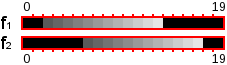
\includegraphics[width=0.4\linewidth]{math_1}}
\caption{Одномерный сдвиг яркостей}
\label{pic:math_1}
\end{figure}

Для начала рассмотрим одномерный случай. Рассмотрим представленные на рисунке \ref{pic:math_1} два одномерных кадра размером 1х20 пикселей. На  рисунке \ref{pic:math_1} кадр $f_2$ смещено вправо на 4 пикселя. Именно это смещение необходимо найти. Для этого представим эти же кадры в виде функций (рисунок \ref{pic:math_2}). На входе позиция пикселя, на выходе — его интенсивность. В таком представление искомое смещение ($d$) видно еще более наглядно. В соответствии с нашим предположением,$f_2$ это просто смещённая $f_1$, то есть можно сказать, что:

\numberwithin{equation}{section}
\label{eq:f_2}
\begin{equation}
f_2(x)=f_1(x-d)
\end{equation}

\begin{figure}[ht]
\center{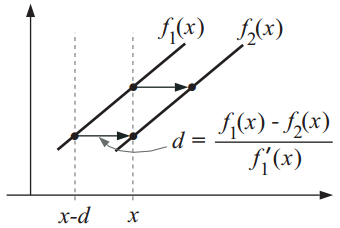
\includegraphics[width=0.4\linewidth]{math_2}}
\caption{Функция зависимости интенсивности от позиции пикселя}
\label{pic:math_2}
\end{figure}

Обратите внимание, что $f_1$ и $f_2$ при желании можно записать и в общем виде: $f_1(x)=I(x,y,t)$ $f_2(x)=I(x,y,t)$ ; где $y$ и $t$ зафиксированы и равны нулю.

Для каждой координаты нам известны значения и в этой точке, кроме того мы можем вычислить их производные. Свяжем известные значения со смещением $d$. Для этого запишем разложение в ряд Тейлора для $f_1(x-d)$:
$$f_1(x-d)=f_1(x)-df^{'}_1(x)+O(d^2f^{''}_1)$$

Сделаем второе важное предположение: Предположим, что достаточно хорошо аппроксимируется первой производной. Сделав это предположение, отбросим всё что после первой производной:
$$f_1(x-d)=f_1(x)-df_1^{'}(x)$$

Насколько это корректно? В общем-то не очень, тут мы теряем в точности, если только наша функция/изображение не строго линейна, как в нашем искусственном примере. Зато это существенно упрощает метод, а для достижения требуемой точности можно сделать последовательное приближение, которе мы рассмотрим позже.

Мы почти у цели. Смещение $d$ — это наша искомая величина. Исходя из \ref{eq:f_2}, сделаем замену:$f_2(x)=f_1(x)-df_1^{'}(x)$
откуда выведем $d = \dfrac{f_1(x)-f_2}{f_1^{'}(x)}$
\subsubsection{Двумерный случай алгоритма}

Теперь перейдём от одномерного случая к двумерному. Запишем разложение в ряд Тейлора для \ref{eq:f_0} и сразу отбросим все старшие производные. Вместо первой производной появляется градиент:
$$I(x+u_x,y+u_y,t+1)=I(x,y,t)+\overrightarrow{u} \nabla I(x,y,t)$$
где $\overrightarrow{u} = \begin{bmatrix}
u_x\\
u_y
\end{bmatrix} $ — вектор смещения.
В соответствии со сделанным допущением \ref{eq:f_0}. Перепишем:
$$I(x,y,t)-I(x_x,y_y,t+1) + \overrightarrow{u} \nabla I(x,y,t) = 0$$
Поскольку между двумя кадрами проходит единичный интервал времени, то можно сказать, что $I(x,y,t)-I(x,y,t+1)$ есть не что иное, как производная по времени.
Заменим:
$$\frac{\partial I(x,y,t)}{\partial t} + \overrightarrow{u} \nabla I(x,y,t) = 0$$
Перепишем ещё раз, раскрыв градиент:
$$\frac{\partial I(x,y,t)}{\partial t} + u_x\frac{\partial I(x,y,t)}{\partial x} + u_y\frac{\partial I(x,y,t)}{\partial y} = 0$$

Мы получили уравнение, которое говорит нам о том, что сумма частных производных должны быть равна нулю. Проблема только в том, что уравнение у нас одно, а неизвестных в нем два: $u_x$ и $u_y$. На этом моменте начинается полет фантазии и разнообразие подходов.

Сделаем третье предположение: Предположим, что смещение пикселей между двумя кадрами невелико. Рассмотрим пиксель $p$, тогда, по алгоритму Лукаса — Канаде, оптический поток должен быть одинаков для всех пикселей, находящихся в окне с центром в $p$. А именно, вектор оптического потока $u_x$ и $u_y$ в точке $p$ должен быть решением системы уравнений. Очевидно, что в общем случае система не имеет решения, поэтому будем искать такие $u_x$ и $u_y$, которые минимизируют ошибку:
$$
\begin{cases}
I_x(q_1) V_x + I_y (q_1) V_y = -I_t(q_1)\\
I_x(q_2) V_x + I_y (q_2) V_y = -I_t(q_2)\\
...\\
I_x(q_n) V_x + I_y (q_n) V_y = -I_t(q_n)\\
\end{cases}
$$
где $q_1,q_2,\dots,q_n$ — пиксели внутри окна
$I_x(q_i),I_y(q_i),I_t(q_i)$ — частные производные изображения $I$ по координатам $x$, $y$ и времени $t$, вычисленные в точке $q_i$.
Это уравнение может быть записано в матричной форме:
$$A v = b$$

$$A = \begin{bmatrix}
I_x(q_1) && I_y(q_1) \\
I_x(q_2) && I_y(q_2) \\
\vdots  && \vdots  \\
I_x(q_n) && I_y(q_n)
\end{bmatrix},
\quad\quad
v =
\begin{bmatrix}
V_x\\
V_y
\end{bmatrix},
\quad\quad
b =
\begin{bmatrix}
-I_t(q_1)\\
-I_t(q_2)\\
\vdots \\
-I_t(q_n)
\end{bmatrix} $$
Полученную переопределенную систему решаем с помощью метода наименьших квадратов. Таким образом, получается система уравнений $2 \cdot 2$:
$$A^T A v=A^T b$$
откуда
$$\mathrm{v}=(A^T A)^{-1}A^T b$$
где $A^T$ — транспонированная матрица $A$. Получаем:
$$\begin{bmatrix} V_x\\[10pt] V_y \end{bmatrix} = \begin{bmatrix} \sum_i I_x(q_i)^2 & \sum_i I_x(q_i)I_y(q_i) \\[10pt] \sum_i I_x(q_i)I_y(q_i) & \sum_i I_y(q_i)^2 \end{bmatrix}^{-1} \begin{bmatrix} -\sum_i I_x(q_i)I_t(q_i) \\[10pt] -\sum_i I_y(q_i)I_t(q_i) \end{bmatrix}$$

Вот собственно и все. Мы знаем приблизительное смещение пикселей между двумя соседними кадрами.

Поскольку в нахождении смещения каждого пикселя участвуют также соседние с ним пиксели, при реализации данного метода целесообразно предварительно посчитать производные кадра по горизонтали и вертикали.
\subsubsection{Недостатки метода}

Описанный выше метод основан на трёх значительных допущениях, которые с одной стороны дают нам принципиальную возможность определить оптический поток, но с другой стороны вносят погрешность. Хорошая новость для перфекционистов состоит в том, что одно допущение нужно нам только для упрощения метода, и с его последствиями мы можем бороться. Мы предполагали, что для аппроксимации смещения нам будет достаточно первой производной. В общем случае это конечно же не так (рисунок \ref{pic:math_3}). Для достижение требуемой точности смещение для каждой пары кадров (назовём их $F_i$ и $F_{i+1}$) можно вычислять итеративно. В литературе это называется искажением (warping). На практике это означает, что, вычислив смещения на первой итерации, мы перемещаем каждый пиксель кадра в противоположную сторону так, чтобы это смещение компенсировать. На следующей итерации вместо исходного кадра $F_{i+1}$ мы будем использовать его искажённый вариант $F_{i+1}^1$. И так далее, пока на очередной итерации все полученные смещения не окажутся меньше заданного порогового значения. Итоговое смещение для каждого конкретного пикселя мы получаем как сумму его смещений на всех итерациях.

\begin{figure}[ht]
\center{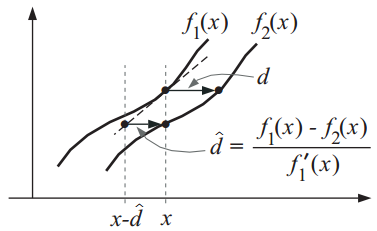
\includegraphics[width=0.4\linewidth]{math_3}}
\caption{Функция зависимости интенсивности от позиции пикселя}
\label{pic:math_3}
\end{figure}

По своей природе данный метод является локальным, то есть при определении смещения конкретного пикселя принимается во внимание только область вокруг этого пикселя — локальная окрестность. Как следствие, невозможно определить смещения внутри достаточно больших (больше размера локальной окрестности) равномерно окрашенных участков кадра. К счастью на реальных кадрах такие участки встречаются не часто, но эта особенность все же вносит дополнительное отклонение от истинного смещения.

\begin{figure}[ht]
\center{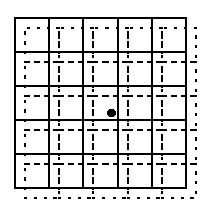
\includegraphics[width=0.4\linewidth]{grid_}}
\caption{Окрестность с субпиксельной точностью}
\label{pic:grid}
\end{figure}

Если интервал времени между кадрами принять за 1, получается следующий алгоритм:
$$\begin{cases} d_k = 0 &\mbox{if } k = 0 \\
d_{k+1}=d_k + C^{-1} \sum_W \left[ (I(x,t) - I(x+d_k,t + 1)) \nabla I (x,t) \right] & \mbox{if } k > 0 \end{cases}
$$
Таким образом, этот алгоритм слежения фактически является поиском точки, в которой достигается минимум некоторой функции, методом градиентного спуска. Во время каждой итерации мы сдвигаемся вдоль направления градиента изображения в текущей точке.
\subsection{Учёт аффинных преобразований}

В этом алгоритме впервые учитываются аффинные искажения изображения окрестности особых точек, поэтому движение пикселей окна особенности описывается в виде $Ax + d$, где $A$ - матрица $(2 \cdot 2)$, $а d$ - смещение $(2 \cdot 1)$.

Задача слежения за особенностью сводится к проблеме проблема определения параметров движения и искажения окна особенности, при которой минимизируется разность:
$$r=\iint_W [J(\Delta x+d)-I(x)]^2$$
где $W$ - окно особенности, а $w$ - весовая функция (может использовать, а может и быть равна 1 во всем окне), $J(x)$ и $I(x)$ - два изображения.

Выражение дифференцируется относительно параметров движения, и производная приравнивается к 0. Затем система линеаризуется с помощью разложения функции изображения в ряд Тейлора:
$$J(\Delta x+d)= J(x)+g^T(u)$$

Это даст нам линейную $6 \cdot 6$ систему:
$$Tz=a$$
, где в векторе $z$ объединены все искомые параметры:

$$z^T=\begin{bmatrix}
 d_{xx} & d_{yx} & d_{xy} & d_{yy} & d_x & d_y
\end{bmatrix}$$
Вектор ошибки a записывается в виде:
$$a=\iint_W [I(x)-J(x)]\begin{bmatrix}
xg_x\\
xg_y\\
yg_x\\
yg_y\\
g_x\\
g_y
\end{bmatrix}\omega dx$$
А матрицу размерности $6 \cdot 6$ $T$ можно представить следующим образом:
$$T=\iint_W [I(x)-J(x)]\begin{bmatrix}
U & V\\
V^T & Z
\end{bmatrix}\omega dx$$

$$U=\begin{bmatrix}
x^3 g^3_x & x^3 g_x g_y & x y g^3_x & x y g_x g_y \\
x^3g_xg_y & x^3g^3_y & xyg_xg_y & xyg^3_x \\
xyg^3_x & xyg_xg_y & y^3g^3_x & y^3g_xg_y \\
xyg_xg_y & xyg^3_y & y^3g_xg_y & y^3g^3_y
\end{bmatrix}$$

$$V^T=\begin{bmatrix}
xg^3_x & xg_xg_y & yg^3_x & yg_xg_y \\
xg_xg_y & xg^3_y & yg_xg_y & yg^3_y
\end{bmatrix}$$

$$Z=\begin{bmatrix}
g^3_x & g_xg_y \\
g_xg_y & g^3_y
\end{bmatrix}$$

Полученная система решается также итеративно по методу Ньютона-Рафсона.

Если движение считается не аффинным, а просто смещением, то первые четыре элемента искомого вектора $z$ обращаются в 0, и значимыми остаются только последние два. Алгоритм превращается в алгоритм Tomasi-Kanade.
\subsection{Пирамидальная версия алгоритма}

Пирамидальная версия или иерархический метод. В данном алгоритме важным является нахождение хорошего начального приближения для вектора скорости. Для этого обычно применяют пирамидальную версию алгоритма. Ее идея заключается в том, что наряду с исходной парой изображений ( f; g ) рассматривают эти же изображения сжатые в два раза ( f 2 ; g 2 ) , в четыре ( f 4 ; g 4 ) и  т.д.  ( пирамида ).  Вектора  скорости находят  сначала  на  самом  верхнем  уровне  пирамиды и затем спускаются вниз этаж за этажом. На самом верхнем уровне в качестве начального приближения берут нулевой вектор. На нижних уровнях за начальное приближение берут удвоенную скорость, полученную на предыдущем шаге. Все это вместе взятое обеспечивает хорошее сочетание скорости, точности и устойчивости алгоритма  нахождения  межкадрового  движения  в  виде сдвигов.

Каждое изображение последовательности, за исключением первого, получается как свёртка предыдущего изображения со следующим фильтром:
(рис. \ref{pic:pyramid}).
Пирамидальный алгоритм Лукаса - Канаде для поиска потока в точке $(x_0,y_0)$.
\begin{enumerate}
\item По каждому из двух данных изображениям строится пирамида изображений
\item Для $i$ – го изображения пирамиды по первому и второму изображениям применяется классический KLT метод, с вектором начального приближения $2 \cdot d_{i+1}$, где $d_{i+1}$ – вектор потока, полученный на предыдущем уровне пирамиды.
\end{enumerate}
Для самого первого уровня этот вектор принимается равным (0,0).

\begin{figure}[ht]
\center{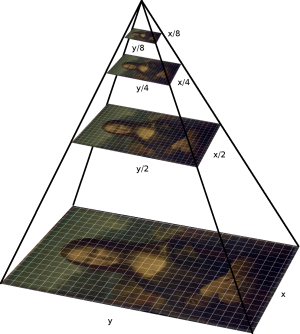
\includegraphics[width=0.6\linewidth]{pyramid}}
\caption{Пример пирамиды Гаусса}
\label{pic:pyramid}
\end{figure}

\subsection{Оценка деформации}

Компоненты рассчитываются путем численного дифференцирования полученного поля смещений. Выражения для продольной $\varepsilon_{xx}$, поперечной $\varepsilon_{yy}$, сдвиговой $\varepsilon_{xy}$ и поворотной $\omega_z$ компонент тензора дисторсии:

$$\varepsilon_{xx}= \frac{\mathrm{d} U_x}{\mathrm{d} x},\varepsilon_{yy}= \frac{\mathrm{d} U_y}{\mathrm{d} y},\varepsilon_{xy}=\frac{1}{2}(\frac{\mathrm{d} U_x}{\mathrm{d} y} + \frac{\mathrm{d} U_y}{\mathrm{d} x}),\omega_z=\frac{1}{2}(\frac{\mathrm{d} U_y}{\mathrm{d} x} - \frac{\mathrm{d} U_x}{\mathrm{d} y})$$

Также выражение для интенсивности деформации сдвига $\gamma_i$

$$\gamma_i = \sqrt\frac{2}{3}\sqrt{(\varepsilon_{xx}-\varepsilon_{xx})^2+\varepsilon_{yy}^2+\varepsilon_{xx}^2 + \frac{3}{2}\varepsilon_{xy}^2}$$
\newpage
\section{Конструкторско-технологическая часть}
\subsection{Сведения о платформе реализации с указанием основных функций операционной системы, необходимых для работы модуля}
\subsection{Обоснование целесообразности разработки оригинальных модулей программного обеспечения}
\subsection{Обоснование выбора технологии программирования и средствразработки}
\subsection{Описание консольного интерфейса программы}% (выбор цветовой палитры экранных форм, расположение элементовуправления на них, использование «горячих» клавиш  акселераторов, выпадающих меню и пр.)}
Интерфейс программы представлен в двух реализациях.
Первый — консольная программа в стиле классического Unix. Интерфейс командной строки более гибкий, позволяет выставить необходимые опции/флаги и запустить программу. Особенности в сравнении с графическим интерфейсом:
\begin{itemize}
\item Интерфейс командной строки позволяет писать скрипты для автоматизации запуска и тестирования с различными входными параметрами, что средствами графического интерфейса гораздо сложнее;
\item Большая функциональность;
\item Некая сложность при использовании, неопытным пользователям;
\item Невозможность просмотра выходных результатов.
\end{itemize}

\begin{figure}[ht]
\center{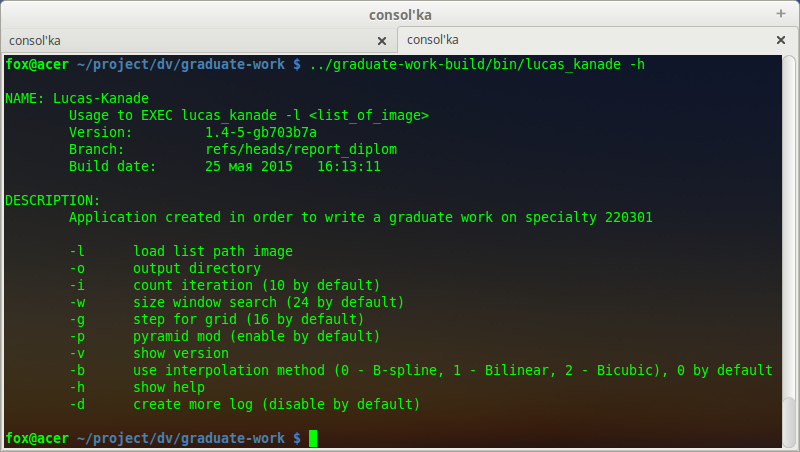
\includegraphics[width=0.8\linewidth]{consol_screen}}
\caption{Пример консольного интерфейса в среде linux}
\label{pic:con_scr}
\end{figure}

\subsubsection{Перечень команд для запуска}
\begin{itemize}
\item l — список изображений для обработки;
\item o — директория для выходных результатов;
\item i — число уточнений при поиске смещенной части (по умолчанию равна 10);
\item w — радиус окна поиска (по умолчанию равна 24);
\item g — шаг между векторами оптического потока(по умолчанию равна 16);
\item p — применить метод пирамды(по умолчанию опция включена);
\item v — показать версию програмного обеспечения;
\item b — использование метода интеполяции(0 — Б-сплайн, 1 — Билинейная, 2 — Бикубическая), по умолчанию 0;
\item h — показать краткую справку;
\item d — генерировать подробный лог файл(по умолчанию опция выключена).
\end{itemize}

\subsection{Описание графического интерфейса программы}
Второй графический — более удобный для неопытного пользователя. 

\begin{figure}[ht]
\center{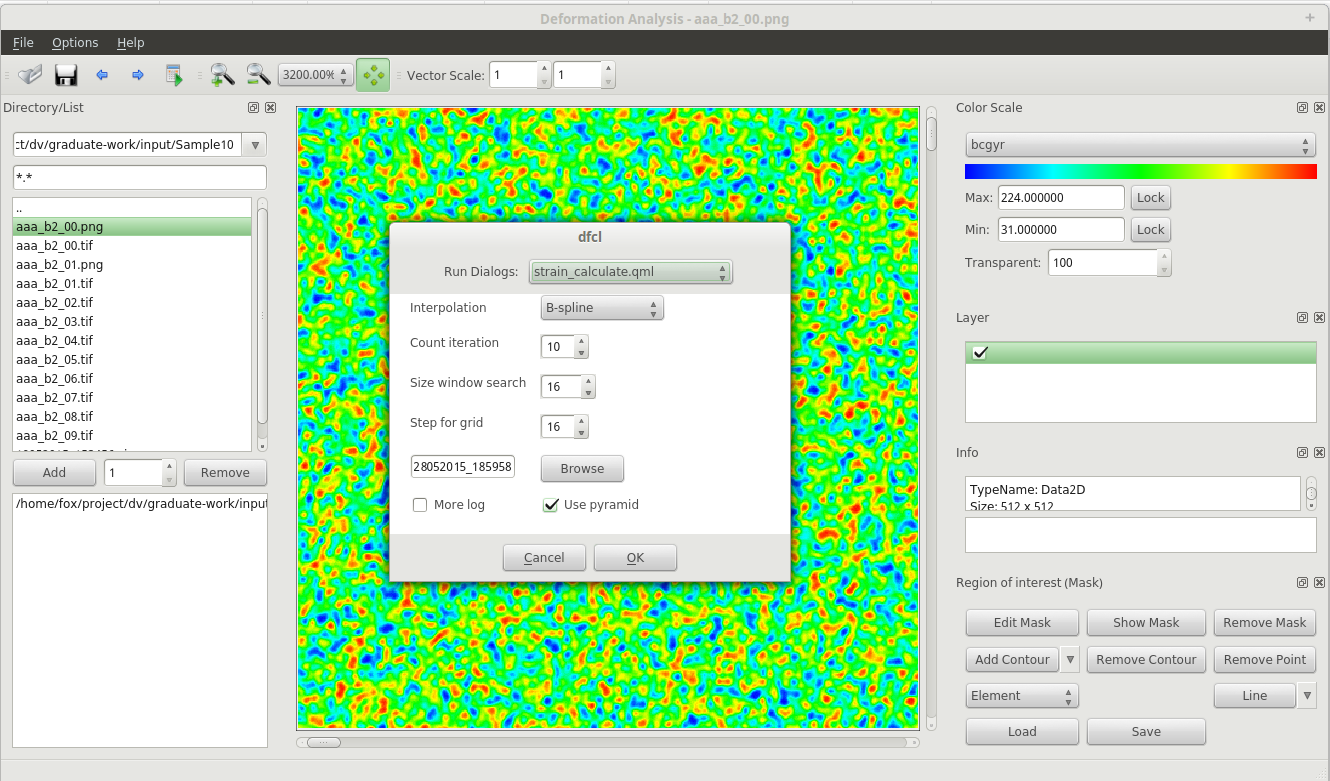
\includegraphics[width=0.8\linewidth]{gui_screen}}
\caption{Пример графического интерфейса}
\label{pic:gui_scr}
\end{figure}

\subsection{Справочную систему пользователя для разрабатываемого модуля,требования к уровню квалификации пользователя}
\subsection{Листинг программы с комментариями, поясняющими работу основных блоков}
\subsection{Блоксхему оригинальных, разработанных автором, алгоритмовработы основных, по мнению автора, программных модулей}
\subsection{Тестовый пример для контроля адекватного функционированияразработанного программного модуля и протокол (листинг) результатов работыпрограммы на этом тестовом примере}
\newpage
\section{Тестирование программного обеспечения}
Эксперименты ставились на парах модельных изображений и на изображениях поверхностях реальных образцов. Для тестирования использовалась следующая конфигурация.
Для корректной работы разрабатываемого программного комплекса, компьютер должен отвечать следующим требованиям:
\subsubsection {Минимальные требования к аппаратному обеспечению}
Минимальные системные требования для операционной системы Linux Debian 8~\cite{debian_8}:

\begin{itemize}
\item процессор 1ГГц Pentium 4;
\item оперативная память 512 Мб;
\item место на жёстком диске -- 9 Гб.
\end{itemize}

Минимальные системные требования для операционной системы Microsoft Windows 7~\cite{windows_7}:

\begin{itemize}
\item процессор 32-разрядный или 64-разрядный 1 ГГц;
\item оперативная память 1 Гб для 32-разрядной системы или 2 Гб для 64-разрядной системы;
\item 16 Гб для 32-разрядной системы или 20 Гб для 64-разрядной системы пространства на жестком диске;
\item графическое устройство DirectX 9 с драйвером WDDM 1.0.

\end{itemize}

\subsubsection {Минимальные требования к программному обеспечению}
Для корректной работы разрабатываемого программного комплекса на компьютере должны быть установлены:
\begin{itemize}
\item Qt5 или Qt4;
\item CMake не ниже 2.8;
\item HDF5 не ниже 1.8.
\end{itemize}
\subsection{Модельные изображения}

В качестве образцов брались наборы изображений из интернет ресурса ``Society for Experimental Mechanics (sem.org)'' описание текстур находится в таблице \ref{tab:set_image}.

\begin{longtable}[h!]{|*7{m{0.12\textwidth}|}}
\caption{Описание используемых серий изображений}
\label{tab:set_image}
\\ \hline
Серия & Имя & Метод & Диапазон яркостей 	& Уровень шума & Сдвиг (px) & Кол-во изображений \\ \hline
Grey texture & Grey set & Shift  & 0-188 & Нет & 1-20 & 5   \\ \hline
HC texture & High contrast & QEM & 10-240 & Низкий  & 0.1-1 & 122  \\ \hline
Prosilica Bin  & Sample6  & Binning & 10-156 & Низкий  & 0.1-1 & 10   \\ \hline
Strain Gradient & Sample11b & FFT & 20-185 	& Средний  & 0.01-1  & 6   \\ \hline
Strain Gradient & Sample10  & FFT & 30-225 	& Средний  & 0.01-1  & 10   \\ \hline
\end{longtable}

\subsection{Реальные отснятые изображения}

В данном разделе приведены результаты тестирования разрабатываемого программного обеспечения на изображениях поверхностей реальных образцов. В экспериментах использовались металлические образцы из авиационного алюминиевого сплава Д16АТ и полимерные образцы из полипропилена, нагружавшиеся на механической испытательной машине ИМАШ-2078 в условиях одноосного статического растяжения.

\begin{figure}[ht]
\center{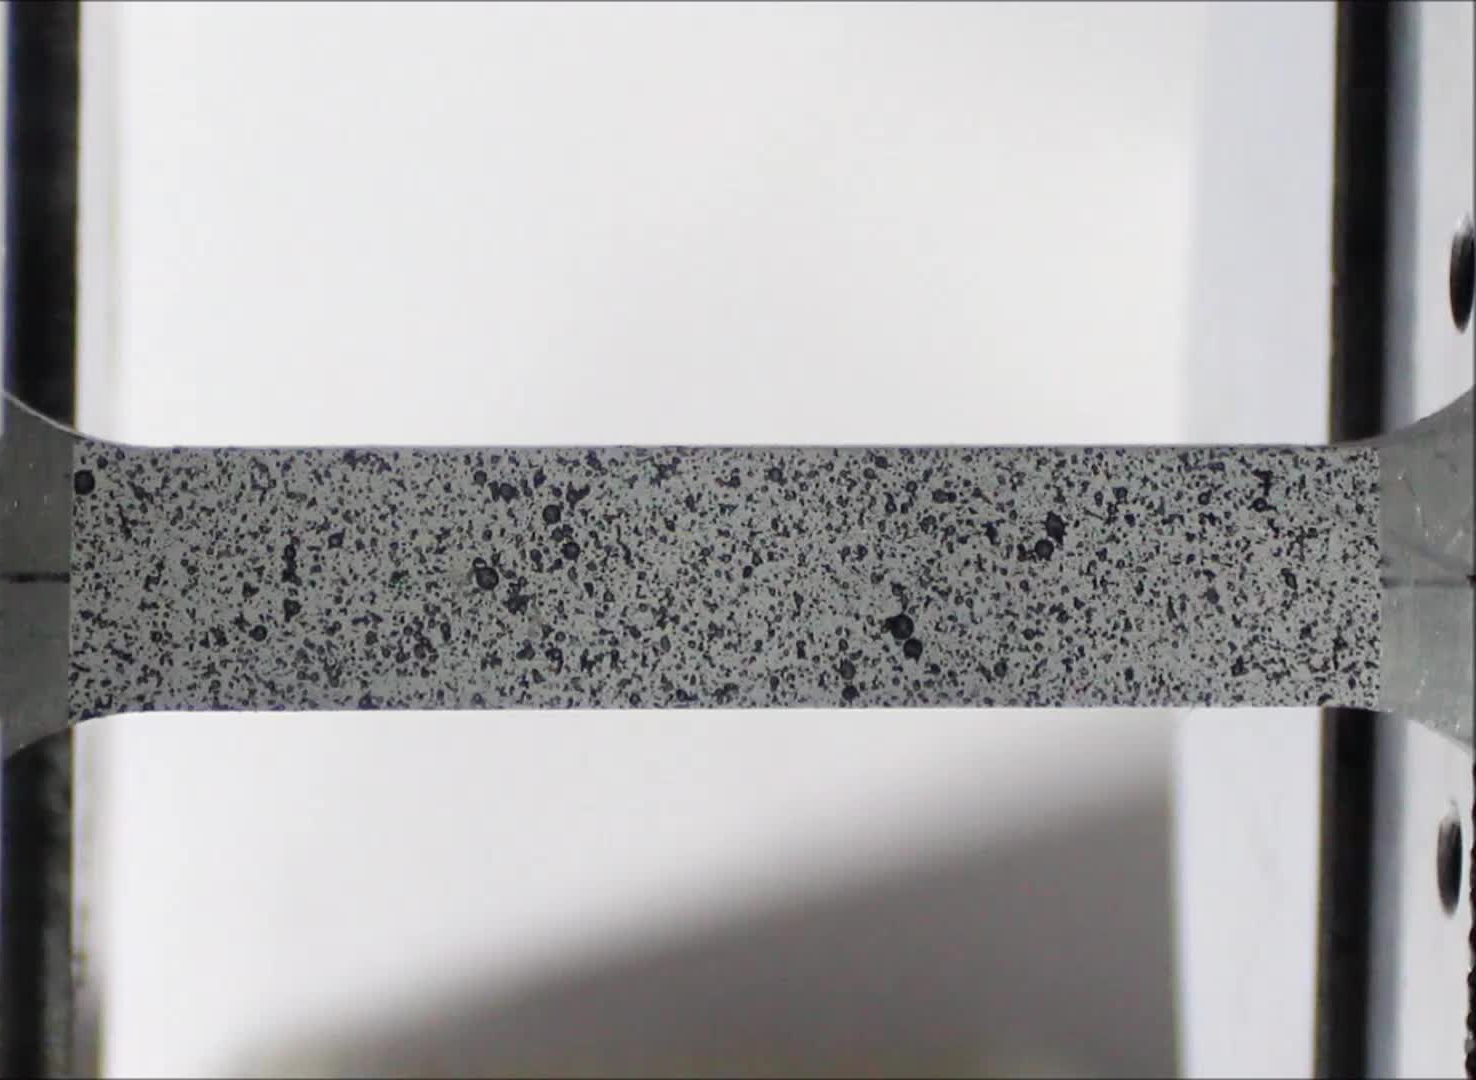
\includegraphics[width=0.6\linewidth]{real_deform}}
\caption{Растяжение пластины алюминия Д16АТ}
\label{pic:real_deform}
\end{figure}

\subsection{Тестирование на модельных изображениях}

Для первого раза используем изображения из серии Grey texture, представленные на рисунке \ref{pic:gray_set}. Они имеют сдвиг по оси $x$ на один пиксель влево, по $y$ сдвиг отсутствует.

\begin{figure}[ht]
\center{
\includegraphics[width=0.6\linewidth]{gray_set}}
\caption{Тестовая серия изображений:Grey texture}
\label{pic:gray_set}
\end{figure}

Результатом работы ПО, как описано в первом разделе, является векторное поле и поля деформации твёрдого тела представленное на рисунке \ref{pic:gray_set_out}.

\begin{figure}[ht]
\center{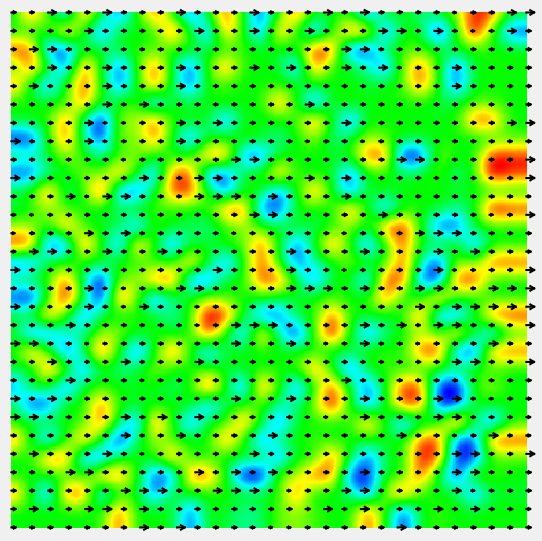
\includegraphics[width=0.6\linewidth]{gray_set_out}}
\caption{Поле смещений и деформации твёрдого тела}
\label{pic:gray_set_out}
\end{figure}

\begin{figure}[ht]
\center{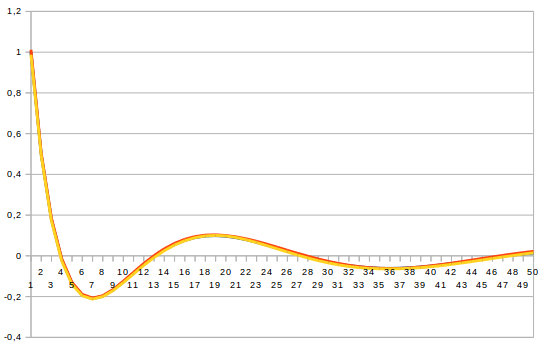
\includegraphics[width=0.6\linewidth]{gray_set_func_iteration}}
\caption{Зависимость уровня ошибки, от числа итераций}
\label{pic:gray_set_func_iteration}
\end{figure}

\begin{figure}[ht]
\center{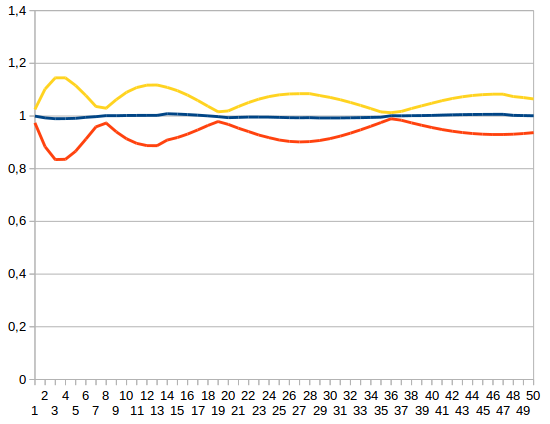
\includegraphics[width=0.6\linewidth]{gray_set_func_iter_vector}}
\caption{Зависимость смещение по x, от числа итераций}
\label{pic:gray_set_func_iter_vector}
\end{figure}

\subsection{Тестирование на экспериментально полученных изображения}
\newpage
\section{Безопасность жизнедеятельности}
\subsection{Анализ опасных и вредных производственных факторов на рабочем месте}
Производственный фактор, воздействие которого на работающего человека, в определённых условиях приводит к травме или другому внезапному резкому ухудшению здоровья, называется опасным. Если же производственный фактор приводит к заболеванию или снижению работоспособности, то его считают вредным (ГОСТ 12.0.002-80).

В зависимости от уровня и продолжительности воздействия вредный производственный фактор может стать опасным.

В целях предупреждения травматизма и профессиональных заболеваний при воздействии опасных и вредных производственных факторов (ОПФ и ВПФ) на предприятиях применяются меры по их предупреждению и устранению, а также снижению степени воздействия на работников.

Согласно ГОСТ 12.0.003 – 74 ``Опасные и вредные производственные факторы. Классификация'', все опасные и вредные производственные факторы делятся по природе воздействия на следующие группы:

\begin{enumerate}
\item физические;
\item химические;
\item биологические;
\item психофизиологические.
\end{enumerate}
Из всех перечисленных факторов в наших условиях работы на организм действуют только физические и психофизиологические опасные и вредные производственные факторы.

К физическим опасным и вредным производственным факторам можно отнести:

\begin{enumerate}
\item недостаточная освещённость помещения. Качество поступающей информации во многом зависит от освещения. Недостаточное освещение не только утомляет глаза, но и вызывает утомление организма в целом. При неудовлетворительном освещении снижается производительность труда и увеличивается брак;
\item повышенное значение напряжения в электрической цепи, замыкание которой может произойти через тело человека. Системный блок и монитор ЭВМ питаются от бытовой сети переменного тока напряжением 220 В частотой 50 Гц;
\item повышенный уровень неионизирующих \ электромагнитных полей и излучений в рабочей зоне;
\item повышенный уровень шума. Одним из важнейших параметров, наносящим ущерб для здоровья и снижающим производительность труда, является шум. Шум может создаваться как работающим оборудованием, установками кондиционирования воздуха, работающими осветительными приборами дневного света, так и проникать извне. Действие шума различно: он затрудняет разборчивость речи, вызывает снижение работоспособности, повышает утомляемость, вызывает необратимые изменения в органах слуха человека. Шум воздействует не только на органы слуха, но и на весь организм человека через центральную нервную систему. Ослабляется внимание, ухудшается память, снижается реакция, увеличивается число ошибок при работе;
\item неудовлетворительное состояние параметров микроклимата. Количество теплоты, выделяемое человеком в окружающую среду, и охлаждающая способность среды должны быть адекватны, то есть человек должен себя чувствовать комфортно. В противном случае у человека возникают беспокоящие его температурные ощущения холода или перегрева, отрицательно сказывающиеся на его самочувствии и работоспособности;
\item возможность возникновения пожара. Во время работы с электрооборудованием в сети переменного тока может возникнуть перегрев и воспламенение самого оборудования или его обшивки.
\end{enumerate}
К психофизиологическим факторам согласно ГОСТ 12.0.003-74 можно отнести такие факторы как:

\begin{enumerate}
\item физические (статические) перегрузки;
\item нервно-психические перегрузки.
\end{enumerate}
В процессе работы инженер не подвержен воздействию химических и биологических производственных факторов.

\subsection{Требования и защитные мероприятия в области БЖД}
\subsubsection{Освещение}
Информация, которую человек получает из внешнего мира, поступает в основном через зрительный канал. Поэтому качество информации, получаемой посредством зрения, во многом зависит от освещения. Неудовлетворительное освещение может исказить информацию; кроме того, оно утомляет не только зрение, но вызывает утомление организма в целом. Неправильное освещение может также, являться причиной травматизма: плохо освещённые опасные зоны, слепящие лампы и блики от них, резкие тени ухудшают или вызывают полную потерю ориентации работающих.

На практике пользуются двумя видами освещения — естественным и искусственным.

При освещении помещений, согласно СНиП 23-05-95 ``Естественное и искусственное освещение'', необходимо соблюдать следующие требования:

\begin{enumerate}
\item естественное освещение должно осуществляться через светопроёмы, ориентированные преимущественно на север и северо-восток, и обеспечивать коэффициент естественной освещённости не ниже 1.2 \%;
\item освещенность рабочего места пользователя ПЭВМ должно быть 200-400 лк (IV (в) разряд зрительных работ, ``Естественное и искусственное освещение СНиП 23-05-95'');
\item для освещения зоны расположения документов допускается установка светильников местного освещения. Местное освещение не должно создавать бликов на поверхности экрана и увеличивать освещённость экрана более 300 лк;
\item в поле зрения оператора должно отсутствовать прямая и отражённая блескость;
\item на рабочем месте оператора должно быть ограничена пульсация освещённости от газоразрядных источников света;
\item в качестве источников света при искусственном освещении должны применяться преимущественно люминесцентные лампы типа ЛБ. Допускается применение ламп накаливания в светильниках местного освещения.
\end{enumerate}
Рассчитаем реальную освещённость на рабочем месте. Целью данного расчёта является проверка соответствия освещённости в рабочем помещении норме освещённости согласно СНиП 23-05-95.

Проведём проверочный расчёт освещённости методом коэффициента использования светового потока.

Освещённость определяется по формуле:
\begin{equation}
\label{eq:sunny}
E=\frac{F{\cdot}N{\cdot}\eta }{k{\cdot}S{\cdot}z}
\end{equation}

где \textit{F} – световой поток каждой из ламп, лм;

\textit{N} – число источников света;

\textit{$\eta $} – коэффициент использования светового потока;

\textit{k} – коэффициент запаса, учитывающий запыление светильников и износ источников света;

\textit{S} – площадь помещения, м\textsuperscript{2};

\textit{z} – коэффициент неравномерности освещения.

Определим данные для расчёта.

Коэффициент \textit{k} для помещений, освещаемых лампами и при условии чистки светильников не реже двух раз в год берётся равным 1,4 – 1,5.

При оптимальном расположении светильников коэффициент неравномерности \textit{z} равен 1,1 – 1,2.

Коэффициент использования светового потока $\eta$ зависит от типа светильника, коэффициента отражения светового потока от стен $\textit{Р}_{\textit{С}}$, потолка $\textit{Р}_{\textit{П}}$, пола $\textit{Р}_{\textit{ПОЛА}}$, а также геометрических размеров помещения и высоты подвеса светильников, что учитывается одной комплексной характеристикой – индексом помещения:

\begin{equation}
\label{eq:index_opt_flor}
I=\frac S{h{\cdot}(A+B)}
\end{equation}

где \textit{h} – высота подвеса светильников над рабочей поверхностью, м;

\textit{А} – ширина помещения, м;

\textit{В} – длина помещения, м.

Рассматриваемое помещение имеет следующие характеристики:

\begin{itemize}
\item ширина \foreignlanguage{english}{\textit{A}} – \foreignlanguage{english}{5} м;
\item длина \foreignlanguage{english}{\textit{B}}\foreignlanguage{english}{ }– 7 м;
\item площадь помещения \foreignlanguage{english}{\textit{S}}\foreignlanguage{english}{ }– 35 м\textsuperscript{2};
\item высота до осветительного прибора \foreignlanguage{english}{\textit{h}} – 3 м;
\item количество ламп \foreignlanguage{english}{\textit{N}} – 8;
\item поправочный коэффициент \foreignlanguage{english}{\textit{Z}} – 1.1;
\item световой поток одной лампы \foreignlanguage{english}{\textit{F}} – 1340 лм;
\item коэффициент запаса \foreignlanguage{english}{\textit{k}} – 0.4.
\end{itemize}
Тогда индекс помещения по формуле (\ref{eq:index_opt_flor}):
%$$ I = \dfrac{S}{h\cdot(A+B)} = \dfrac{35}{3\cdot\(5+7\)} = 0.97$$
Используя этот коэффициент по светотехнической таблице, находим, что для нашего помещения коэффициент \textit{$\eta $ }равен 53 \%.

Теперь можно произвести расчёт освещённости по формуле (\ref{eq:sunny}):

$$
%E=\dfrac{F\cdot N \cdot \eta}{k \cdot S \cdot z} = \dfrac{1340{\cdot}8{\cdot}0.53}{35{\cdot}1.1{\cdot}0.4}=369
$$
Согласно СНиП 23-05-95, освещённость рассматриваемого помещения находится в диапазоне оптимального освещения, т.к. по нормативам для разряда зрительной работы \foreignlanguage{english}{IV} (\textit{в}) норма освещённости находится в диапазоне от 200 лк до 400 лк. Это означает, что мощность и количество осветительных приборов для данного помещения выбраны правильно, и не требуется дополнительного освещения.
\subsubsection{Микроклимат}

Выбор типа \textit{производственного помещения} определяется технологическим процессом, возможностью борьбы с шумом, вибрациями и загрязнением воздуха. Наличие больших оконных проёмов и фонарей должно обеспечивать хорошую естественную освещённость. В помещении обязательно устройство вентиляции.

Объем и площадь производственного помещения, которые должны проходиться на каждого работающего по санитарным нормам, должны быть не менее 20 $m^{3}$ и 6 $m^{2}$ соответственно. Высота производственных помещений не должна быть менее 4 м. Стены и потолки необходимо сооружать из малотеплопроводных материалов, не задерживающих осаждение пыли. Полы должны быть тёплыми, эластичными, ровными и нескользкими.

Под оптимальными микроклиматическими условиями понимают такие сочетания параметров микроклимата, которые при детальном и систематическом воздействии на человека обеспечивают сохранение нормального функционального и теплового состояния организма.

На организм человека и работу вычислительной техники большое влияние оказывает относительная влажность воздуха. При влажности воздуха до 40\% становится хрупкой основа магнитной ленты, повышается износ магнитных головок, выходит из строя изоляция проводов, также возникает статическое электричество при движении носителей информации в ЭВМ. При относительной влажности воздуха более 75-80\% снижается сопротивление изоляции, изменяются рабочие характеристики ЭВМ, возрастает интенсивность их отказов.

Скорость движения воздуха тоже оказывает влияние на функциональную деятельность человека, так как способствует испарению влаги с кожного покрова. А это, в свою очередь, приводит либо к высыханию кожи, либо к нарушению теплового равновесия организма, т.е. скорость движения воздуха, может иметь положительное значение с точки зрения физического охлаждения лишь до температуры воздуха $35-36^{\circ} C$. При дальнейшем повышении температуры окружающей среды единственным путём теплопередачи является испарение. Однако при повышении температуры свыше $40^{\circ} C$ движение даже относительно сухого воздуха может оказываться неблагоприятным фактором. Горячий воздух отдаёт теплоту телу, и подвижность воздуха в этом случае приводит не к охлаждению, а, наоборот, к нагреванию.

В машинном зале рекомендуется поддерживать температуру и влажность воздуха постоянными. Атмосферное давление должно быть в допустимых пределах, так как при пониженном, например, давлении ухудшается отвод тепла от элементов ЭВМ, снижаются изоляционные свойства узлов и устройств ЭВМ.

Воздух должен в значительной степени очищаться от пыли. ЭВМ, имеющие в своём составе устройства ввода-вывода на магнитных дисках, требуют этого, так как пылинки, попадающие на рабочую поверхность диска, могут привести к повреждению магнитной головки или поверхности диска. Пыль, оседающая на устройства и узлы ЭВМ, ухудшает теплоотдачу, может образовывать токопроводящие цепи, вызывает износ подвижных частей, нарушает контакты и приводит к засорению лёгких у работающего персонала.

Не менее важно и значение освещения. При неудовлетворительном освещении зрительная способность снижается, и могут появиться заболевания глаз. Правильно выполненная система освещения имеет большое значение в снижении травматизма, уменьшая потенциальную опасность многих производственных факторов; создаёт нормальные условия для работы органов зрения и повышает общую работоспособность организма.

С целью создания нормальных условий работы установлены нормы производственного микроклимата (ГОСТ 12.1.005-88). Эти нормы устанавливают оптимальные и допустимые значения температуры, относительной влажности и скорости движения воздуха для рабочей зоны помещений, оборудованных компьютерами с учётом тяжести выполняемой работы и сезона года.

\begin{table}[!ht]
\centering
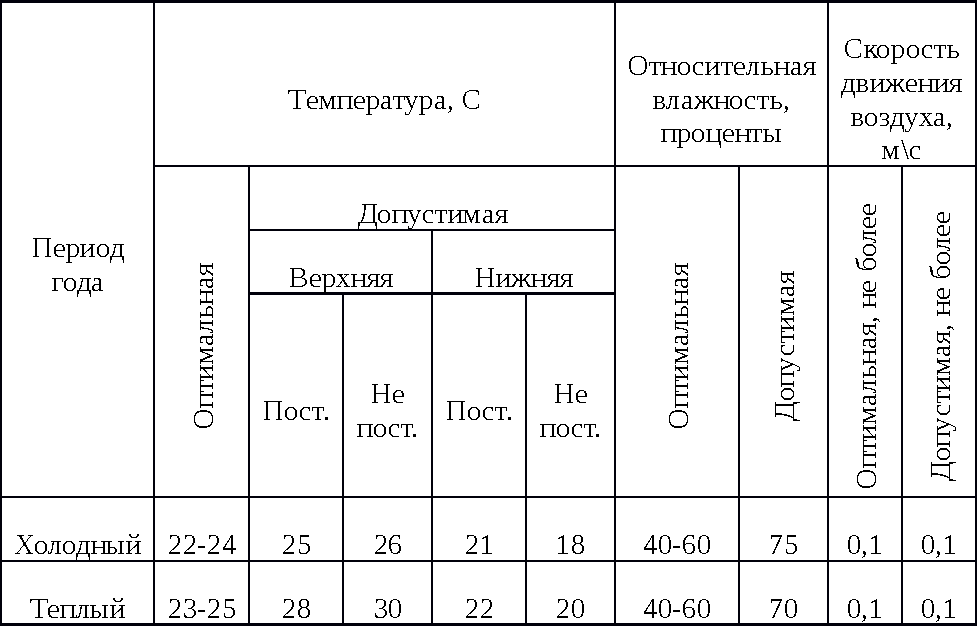
\includegraphics[width=1\linewidth]{voltage_amper.pdf}
\caption{Оптимальные и допустимые нормы температуры, относительной влажности и скорости движения воздуха в рабочей зоне производственного помещения}
\label{tab:micro_climat}
\end{table}

\subsubsection{Электробезопасность}

Электрические установки, к которым относится ЭВМ и стенд, представляют для человека потенциальную опасность. В процессе эксплуатации или при проведении профилактических работ человек может соприкасаться с частями, находящимися под током. Согласно классификации помещений по электробезопасности (ПУЭ – 7-е издание) рабочий кабинет относится к помещениям без повышенной опасности, характеризующимся наличием следующих условий:

\begin{enumerate}
\item напряжение питающей сети, 220 В;
\item напряжение питающей сети, 380 В;
\item относительная влажность воздуха, не более $75\%$;
\item средняя температура не более $25^{\circ}C$;
\end{enumerate}
При нормальном режиме работы опасность поражения электрическим током невелика, однако, возможны режимы, называемые аварийными, когда происходит случайное электрическое соединение частей оборудования, находящихся под напряжением с заземлением конструкциями. Опасность поражения электрическим током существует всюду, где используются электроустановки, поэтому помещения без повышенной опасности нельзя назвать безопасными.

Любое из воздействий тока (термическое, электролитическое, механическое и биологическое) может привести к электрической травме, т. е. к повреждению организма, вызванному действием электрического тока или электрической дуги.

Основными техническими способами и средствами защиты от поражения током, согласно ГОСТ 12.1.019-79 ``Система стандартов безопасности труда. Электробезопасность. Общие требования и номенклатура видов защиты'', являются: защитное зануление, выравнивание потенциалов, защитное заземление, электрическое разделение сети, изоляция токоведущих частей, оградительные устройства и другое.

Согласно ``Система стандартов безопасности труда. Электробезопасность. Предельно допустимые значения напряжений прикосновения и токов'' ЭВМ и стенд, на которых производится работа, относятся к классу электробезопасности 01 (имеет рабочую изоляцию, элемент для заземления и провод без заземляющей шины для подключения питания).

Напряжения прикосновения и токи, протекающие через тело человека при нормальном (неаварийном) режиме электроустановки не должны превышать значений, указанных в таблице \ref{tab:voltage_amper}

\begin{table}[h]
\centering
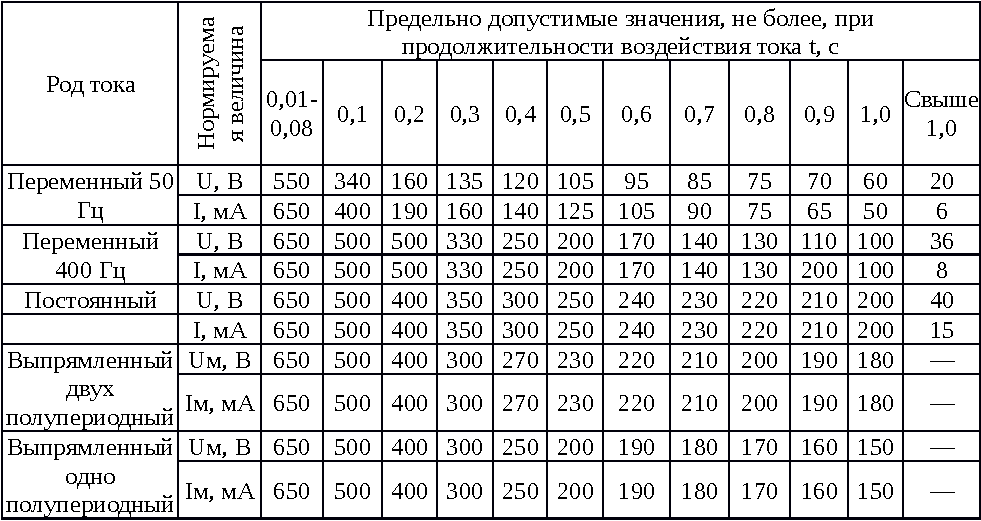
\includegraphics[width=1\linewidth]{in-crop.pdf}
\caption{Таблица предельно допустимых значений напряжений прикосновения и токов}
\label{tab:voltage_amper}
\end{table}

Для исключения возможности поражения электрическим током проведены следующие меры:

\begin{enumerate}
\item токоведущие части, находящиеся под напряжением, изолированы;
\item корпуса приборов заземлены;
\item заземляющие проводники видны, а места их соединений скреплены резьбовыми соединениями.
\end{enumerate}
\subsubsection{Пожарная безопасность}

Для выполнения требований по пожарной безопасности (ГОСТ 12.1.004-91 ССБТ. Пожарная безопасность) необходимо удаление оборудования друг от друга на расстояние не менее 60-80 см.

Опорные части из изоляционных материалов, удерживающие детали, предназначенные для подключения к сети, а также изолирующие корпуса должны быть изготовлены из материалов, не представляющих опасность при возникновении коротких замыканий внутри блока или при нагреве, вызываемого плохим контактом внешних проводов.

Необходимо также наличие пожарного инвентаря и проведение инструктажей.

Приведём возможные причины возникновения пожаров:
\begin{enumerate}
\item наличие твёрдых горючих веществ;
\item опасная перегрузка сетей, которая ведет за собой сильный разогрев токопроводящих проводников и загорания изоляции;
\item короткие замыкания;
\item пуск оборудования после ремонта.
\end{enumerate}
Для предупреждения пожаров от коротких замыканий, перегрузок необходим правильный выбор монтаж и соблюдение установленного режима эксплуатации электрических сетей, дисплеев и других устройств.

\subsubsection{Электромагнитные неионизирующие излучения}

Длительное воздействие электромагнитных полей промышленной частоты (50 Гц) приводит к расстройствам в головном мозге и центральной нервной системе. В электрическом поле (ЭП) атомы и молекулы поляризуются.
Полярные молекулы ориентируются по направлению распространения электромагнитного поля, что изменяет ориентацию клеток или цепей молекул, ослабляя биохимическую активность белковых молекул.
В результате у человека наблюдаются головная боль в височной и затылочной областях, вялость, ухудшение памяти, боли в области сердца, угнетённое настроение, апатия, своеобразная депрессия с повышенной чувствительностью к яркому свету и интенсивному звуку, расстройство сна, сердечно-сосудистой системы (ССС), органов пищеварения, дыхания, повышенная раздражительность.
Могут наблюдаться функциональные нарушения в ЦНС, а также изменения в составе крови.

Воздействие постоянного магнитного поля (ПМП) и с частотой 50 Гц на человека проявляется в индуцировании в теле человека вихревых токов.

При длительном систематическом воздействии могут возникнуть изменения функционального состояния нервной системы, иммунной системы и сердечно-сосудистой системы. Длительное воздействие ЭМП промышленной частоты может спровоцировать онкологические заболевания.

Предельно допустимые значения напряжённости электрического и магнитного полей промышленной частоты в зависимости от времени их воздействия устанавливаются СанПиН 2.2.4.1191-03 “Электромагнитные поля в производственных условиях”. Согласно этому нормативному документу пребывание в ЭП промышленной частоты напряжённостью до 5 кВ/м допускается в течение всего рабочего дня.

При работе на персональном компьютере расстояние от монитора до глаз пользователя должно быть не менее 50 см. Исследования показали, что с уменьшением расстояния на каждые 10 см уровень электромагнитного излучения возрастает в среднем в 1,5 раза, а с увеличением расстояния с 50 до 60 см уменьшение уровня электромагнитного поля идет в той же зависимости.

Таблица 7.  - Допустимые значения параметров неионизирующих электромагнитных излучений(в соответствии с СанПиН 2.2.2.542-96)

\begin{table}[h]
\begin{longtable}[!ht]{|m{0.75\textwidth}|m{0.15\textwidth}|}
%\begin{longtable}{|l|l|}
\caption{Допустимые значения параметров неионизирующих электромагнитных излучений}
\label{tab:min_neoinige_elwave}
\\ \hline
Наименование параметра & Допустимые \\ \hline
Напряжённость электрической составляющей электромагнитного поля на расстоянии 50см от поверхности видеомонитора & 10В/м\\ \hline
Напряжённость магнитной составляющей электромагнитного поля на расстоянии 50см от поверхности видеомонитора & 0,3А/м\\ \hline
Напряжённость электростатического поля не должна превышать: для взрослых пользователей & 20кВ/м\\ \hline
для детей дошкольных учреждений и учащихся средних специальных и высших учебных заведений & 15кВ/м\\ \hline
\end{longtable}
\end{table}

\subsubsection{Допустимые уровни звукового давления и звукового шума}

Шум на исследовательском рабочем месте создаётся вентиляционной системой ПЭВМ и печатающим устройством. В процессе рабочего дня принтер включается по мере необходимости, поэтому шум следует квалифицировать как непостоянный, прерывистый.

Основными физическими величинами, характеризующими шум, являются интенсивность, звуковое давление и частота. Согласно ГОСТ 12.1.003-83 ``Система стандартов безопасности труда. Шум. Общие требования безопасности'' для оценки шума используют частотный спектр измеряемого уровня звукового давления, выраженного в дБ, в октавных полосах частот, который сравнивают с предельным спектром, приведены в таблице \ref{tab:arm_noise_locate}.

\begin{table}[h]
\begin{longtable}{|l|l|l|l|l|l|l|l|l|l|}
\caption{Значения предельно допустимых уровней шума на рабочих местах производительных предприятий}
\label{tab:arm_noise_locate}
\\ \hline
Рабочие места & \multicolumn{8}{l|}{\begin{tabular}[c]{@{}l@{}}Уровни\\ звукового давления, дБ,,в\\ октавной полосе частот, Гц\end{tabular}} & \begin{tabular}[c]{@{}l@{}}Уровни\\ звука, дБ\end{tabular} \\ \cline{2-10}
                               & 63           & 125           & 250           & 500           & 1000          & 2000          & 4000          & 8000          &                                                            \\ \hline
(1)                            & 71           & 61            & 54            & 49            & 45            & 45            & 40            & 38            & 50                                                         \\ \hline
(2)                            & 79           & 70            & 63            & 58            & 55            & 55            & 50            & 49            & 60                                                         \\ \hline
(3)                            & 83           & 74            & 68            & 63            & 60            & 60            & 55            & 54            & 65                                                         \\ \hline
(4)                            & 94           & 87            & 82            & 78            & 75            & 75            & 71            & 70            & 80                                                         \\ \hline
(5)                            & 99           & 92            & 86            & 83            & 80            & 78            & 76            & 74            & 85                                                         \\ \hline
\end{longtable}
\end{table}

(1) – помещение технологических бюро, лаборатории для теоретических работ;

(2) – помещения управлений, рабочие комнаты;

(3) – кабины наблюдения и дистанционного управления с речевой телефонной связью, помещение и участки тонкой сборки;

(4) – лаборатории для проведения экспериментальных работ;

(5) – постоянные рабочие места и рабочие зоны в производственных помещениях и на территории предприятий.

Уровень шумов от компьютеров и вентиляторов в помещении соответствует пункту (1) таблицы 7.2.3. Согласно ГОСТ 12.1.003-83 шум, создаваемый вентиляторами и компьютерами, постоянный и не превышает установленного звукового давления.

\subsection{Требования эргономики и технической эстетики}
Для создания благоприятных условий труда в лаборатории необходимо учитывать психофизические особенности человека, а также общую гигиеническую обстановку. Большое значение в создании оптимальных условий труда имеют складывающиеся в трудовом коллективе взаимоотношения между студентами, которые принято называть социальным климатом. Человек, находящийся в состоянии нервного возбуждения допускает много ошибок при работе с технологической документацией.

С эстетической точки зрения помещение и оборудование должны быть окрашены в спокойные тона (синие, голубые, зелёные) успокаивающие и уменьшающие зрительное утомление. Окраска стен и дверей помещения должна иметь мягкие переходы без резких яркостных контрастов. В рабочем помещении стены покрашены бежевой краской, потолок покрыт белой плиткой, двери окрашены в синий цвет. Это даёт хорошее отражение и рассеяние света.

Важную роль играет планирование рабочего места, которое должно удовлетворять требованиям удобства выполнения работ и экономии энергии, времени инженера, удобства обслуживания устройств ЭВМ и соблюдения правил охраны труда. Рабочее место должно обеспечивать удобство выполнения работы в помещении сидя, стоя и соответствовать требованиям ГОСТ 12.2.032-78 и ГОСТ 12.2.033-78. Необходим учёт эргономических свойств человека, подбор вспомогательных предметов оборудования (столы, и т. п.), удобных для использования на рабочем месте. Для этого требуется рациональная расстановка оборудования, оптимальная организация рабочего места (правильный выбор основного технологического оборудования, удобство выполнения работ). Рабочее место при выполнении действий в положении сидя должно соответствовать нормам ГОСТ 12.2.032-78.

Определим требования к рабочему месту: обеспечение возможности удобного выполнения работ, учёт физической тяжести труда, учёт размеров рабочей зоны, учёт технологических особенностей процесса выполнения работ. Параметры рабочего места инженера приведены в таблице \ref{tab:arm_ing_locate}.

\begin{longtable}[!ht]{|m{0.4\textwidth}|m{0.2\textwidth}|m{0.2\textwidth}|}
\caption{Параметры рабочего места инженера}
\label{tab:arm_ing_locate}
\\ \hline
Параметры &  Рекомендуемые, мм &  Фактические, мм\\\hline
Высота сидения &  450 &  440\\\hline
Высота рабочей поверхности &  720 &  700\\\hline
Ширина сидения &  500 &  490\\\hline
Высота спинки сидения &  800 &  740\\\hline
Высота пространства для ног &  600 &  700\\\hline
Размеры рабочей поверхности &  1600x900 &  1600x1000\\\hline
Высота ПК &  620x800 &  740\\\hline
Расстояние от глаз инженера до предмета &  600 &  620\\\hline
Расстояние от экрана или предмета до края стола &  750 &  650\\\hline
\end{longtable}

В рабочей зоне необходимо исключение резких и подвижных теней, отблесков. При планировке рабочего места необходимо учитывать зоны досягаемости рук оператора при расположении дисплея, клавиатуры, органов управления системы и периферийных устройств. Эти зоны, установленные на основании антропометрических данных человеческого тела, дают возможность рационально разместить как по горизонтали, так и по вертикали все элементы рабочего места.

Правильная организация рабочего места оператора ЭВМ предусматривает также соблюдение следующих параметров:

\begin{enumerate}
\item высота мыши с клавиатурой (62-88) см (над уровнем пола);
\item высота экрана (над уровнем пола) (90-128) см;
\item расстояние от экрана до края стола (0-115) см;
\item наклон экрана от минус $15\textsuperscript{0}$ до плюс $20\textsuperscript{0}$ к нормальному его положению;
\item расстояние от глаз оператора до экрана должно быть в пределах от 40 до 80 см.
\end{enumerate}
В состав рабочего места входят учебный стенд, персональный компьютер, видеомонитор, клавиатура.

Органы управления, к которым относятся клавиатура и манипулятор ``мышь'' ЭВМ \ \ расположены в зоне досягаемости, ограниченной длиной руки, т.е. от 70 до 80 см. Такое расположение обеспечивает равномерную нагрузку обеих рук оператора.

К системам отображения информации, на данном рабочем месте, относятся: видеомонитор ЭВМ. Видеомонитор распложён в зоне пространства отображения информации ($\pm15^{\circ}C$ от нормальной линии взгляда), что обеспечивает оптимальный зрительный поиск.

В результате анализа можно сделать вывод, что организация рабочего места, на котором выполнялась дипломная работа, удовлетворяет перечисленным выше требованиям правильной организации рабочего места оператора ЭВМ. Так, как и остальные условия работы в помещении являются удовлетворительными (микроклимат, освещение и т.д.), о чем писалось выше, то согласно ГОСТ 12.2.032-78.ССБТ данное рабочее место работника можно считать соответствующим общим эргономическим требованиям.

\subsection{Общие требования безопасности перед началом, вовремя, по окончании работы и в случае аварийных ситуаций}
\subsubsection{Требования безопасности перед началом работы}

Перед началом работы работник должен:

\begin{itemize}
\item проверить на рабочем месте наличие и пригодность средств защиты, инструмента и приспособлений, а также наличие электрического фонаря, средств пожаротушения, плакатов или знаков безопасности;
\item проверить достаточность освещения рабочей зоны и на обслуживаемом оборудовании (отсутствие перегоревших ламп) наличие плафонов на светильниках;
\item ознакомиться с работами производимыми предыдущими работниками, прочитав об этом в ``Оперативном журнале'';
\item при обнаружении, каких-либо отклонений в работе САР доложить технику.
\end{itemize}
\subsubsection{Требования безопасности во время работы}
\begin{itemize}
\item использовать инструмент и приспособления, предназначенные только для выполнения данной работы. Не допускать применения случайных приспособлений и предметов вместо инструмента;
\item следует выполнять только ту работу, которая поручена;
\item импульсные трубопроводы, на которых производится ремонт оборудования КИПиА, необходимо перекрыть при помощи запорной арматуры и снять давление;
\end{itemize}
Запрещается во время работы:

\begin{itemize}
\item \begin{itemize}
\item \begin{itemize}
\item эксплуатировать неисправное оборудование, а также оборудование с неисправными или отключёнными устройствами аварийного отключения блокировок, защит и сигнализации;
\item применять для отмывки и обезжиривания деталей и оборудования керосин, бензин, бензол, ацетон и другие, горючие и легковоспламеняющиеся вещества, при уборке помещений и оборудования горючие вещества, а также хлорпроизводные углеводороды;
\end{itemize}
\end{itemize}
\end{itemize}
\begin{itemize}
\item при обнаружении дефектов на оборудовании немедленно сообщить об этом своему руководству и руководству обслуживаемого объекта;
\item во время работы необходимо поддерживать чистоту и порядок на рабочем месте;
\item во время работы соблюдать противопожарные правила, знать местонахождение первичного противопожарного инвентаря, уметь его применять и не допускать использование противопожарных средств не по назначению;
\end{itemize}
\subsubsection{Действия в аварийных ситуациях}

При возникновении аварии или ситуации, которые могут привести к нежелательным последствиям, необходимо прекратить работу, принять меры по предупреждению несчастных случаев, выхода из строя оборудования, сообщить технику или заведующему кафедры, в котором возникла аварийная ситуация, а также принять меры обеспечения безопасности других лиц;

При возникновении аварийных ситуаций необходимо:

\begin{itemize}
\item прекратить работу;
\item обесточить оборудование, если это угрожает жизни и здоровью персонала;
\item принять меры по предупреждению несчастных случаев, выхода из строя оборудования;
\item сообщить руководству;
\end{itemize}

\begin{itemize}
\item при возникновении пожара необходимо немедленно вызвать пожарную охрану, отключить электрооборудование, находящееся в зоне пожара. Приступить к тушению пожара с помощью первичных средств пожаротушения. Для тушения пожара в электроустановках необходимо применять только углекислотные и порошковые огнетушители.
\end{itemize}
\subsubsection{Требования безопасности по окончании работы}

По окончании работы работник должен:

\begin{itemize}
\item выключить оборудование;
\item привести в порядок рабочее место.
\end{itemize}
\newpage
\section{Технико-экономическое обоснование}
\subsection{Обоснование необходимости проводимого исследования}

Настоящая дипломная работа исследует реализацию дифференциального алгоритма Лукаса-Канаде ?и его вариации? для поиска смещений по парам изображений. На основе полученных векторных полей смещений можно строить карты поверхностной деформации твердого тела. 

Целью данной работы является создание программного обеспечения для анализа оптических изображений поверхности материалов, выявление скорости и точности работы алгоритма Лукаса-Канаде в зависимости от окна поиска и метода аппроксимации при суб-пиксельном смещении изображения.

Продолжение исследований по данной тематике может привести к ХХХХХХХХХХХХХХХХХХХХХХХХХХХХХХХХХХХХХХХХХХХХХХХХХ.
\subsection{Планирование комплекса работ по разработке программного обеспечения}
Основными задачами планирования работ являются:
\begin{enumerate}
\item определение объема предстоящих;
\item распределение объема работ на взаимосвязанные последовательные этапы;
\item установление сроков выполнения работ;
\item определение необходимых, для выполнения планируемых работ денежных, материальных и трудовых ресурсов.
\end{enumerate}
При выполнении дипломной работы было задействовано два человека:
\begin{enumerate}
\item руководитель (рук.);
\item разработчик (разр.).
\end{enumerate}
Руководитель выполняет контроль выполнения различных этапов работ, согласованность этапов выполнения работ между собой, корректирует действия разработчика, дает рекомендации по выполнению тех или иных работ. Разработчик реализует тот объем работ, который установлен руководителем в соответствие с техническим заданием.

Месячный оклад студента в ТУСУР равен 1430 рублей, с учетом 21 рабочих дней в месяце, и 8 часового рабочего дня, стоимость одного часа работ равна 8,5 рублей. Месячный оклад руководителя д.н., профессора в университете равен 14800 рублей, с учетом 24 рабочих дней, и 6 часового рабочего дня, стоимость одного часа работ равна 102,8 рубля. [Приказ ректора от 22.03.2013 г. № 3106. С изменениями от 09.12.2013 г. № 14249]

График выполнения работ приведен в таблице 1.1.

Зная длительность цикла каждого этапа и возможность их параллельно-последовательного выполнения, можно рассчитать срок завершения планируемых работ и составить ленточный и сетевой графики плана их выполнения. Поскольку работа не требует большого состава исполнителей, то ограничимся ленточным графиком планирования, представленным в виде таблицы 1.2.

Таблица 1.2 – Ленточный график загрузки участников работ

\subsection{Определение сметной стоимости проекта}
\subsubsection{Общие положения}
Смета затрат для данной работы состоит из расходов, которые включают в себя следующие статьи:
\begin{enumerate}
\item затраты на оборудование и амортизацию;
\item расходы на оплату труда и отчисления на социальные нужды;
\item затраты на основные и вспомогательные материалы;
\item затраты на электроэнергию.
\end{enumerate}
\subsubsection{Затраты на оборудование и амортизацию}
Основным оборудованием при проведении работы являются компьютер и принтер, которые постановлением Правительства Российской Федерации от 1.01.02 г. N 1 отнесены ко второй амортизационной группе – «имущество со сроком полезного использования свыше 2 лет до 3 лет включительно». Месячная норма амортизации составляет 2,8\% и для компьютера, и для принтера.
Результаты расчетов амортизационных отчислений приведены в таблице 1.3.
Таблица 1.3 – Смета затрат на оборудование
\subsubsection{Расходы на оплату труда и отчисления на социальные нужды}
Статья затрат учитывает выплаты по заработной плате за выполненную работу, исчисленные на основании тарифных ставок и должностных окладов в соответствии с принятой в организации-разработчике системой оплаты труда. В этой статье также отражаются премии, надбавки и доплаты за условия труда, оплата ежегодных отпусков, выплата районного коэффициента и некоторые другие расходы. Отчисления на социальные нужды учитывают страховые взносы.
Результаты расчета расходов на оплату труда участников проекта представлены в таблице 1.4.
Таблица 1.4 – Расчет расходов на оплату труда участников проекта
\subsubsection{Затраты на основные и вспомогательные материалы}
Статья включает расходы по приобретению и доставке основных и вспомогательных материалов, необходимых для опытно-экспериментальной проработки решения, для изготовления макета или опытного оборудования. Сюда включаются и стоимость необходимых материалов для изготовления образцов и макетов, и материалов необходимых для оформления требуемой документации. 
Размер транспортно-заготовительных расходов (ТЗР), определяемый в процентах от стоимости, примем 10\%. Стоимость вспомогательных материалов принимается 10\% от стоимости основных материалов с учетом ТЗР. Результаты расчета стоимости материалов представлены в таблице 1.5.
Таблица 1.5 – Смета затрат на основные и вспомогательные материалы
\subsubsection{Расходы на электроэнергию}
Статья включает затраты по электроэнергии на технологические нужды. В настоящее время тариф на электроэнергию для населения г. Томска на 2015 год составляет 2,7 руб./ кВт ч. Введённый приказом от 26.12.2014 №6/9 (691) ``О тарифах на электрическую энергию для населения и потребителей, приравненных к категории население по Томской области на 2015 год'', принятый департаментом тарифного регулирования Томской области.
Результаты расчетов приведены в таблице \ref{tab:zatr_elek}.
\begin{longtable}[h!]{|*6{m{0.14\textwidth}|}}
\caption{Затраты на электроэнергию}
\label{tab:zatr_elek}
\\ \hline
Наименование оборудования & Количество, шт. & Потребляемая мощность, кВт & Часы работы & Тариф за,1 час, руб. & Стоимость электроэнергии, руб. \\ \hline
Ноутбук                               & 1               & 0,05                       & 560         & 2,7                  & 74,6                           \\ \hline
Принтер                               & 1               & 0,1                        & 4           & 2,7                  & 1,08                           \\ \hline
Освещение                             & 1               & 0,6                        & 560         & 2,7                  & 907,2                          \\ \hline
\multicolumn{6}{|l|}{Всего: 983,88 руб.} \\ \hline
\end{longtable}

\subsubsection{Накладные расходы}
Расчёт накладных расходов сведём в таблицу \ref{nakl_rash}.

\begin{longtable}[h!]{|*4{m{0.22\textwidth}|}}
\caption{Накладные расходы}
\label{tab:nakl_rash}
\\ \hline
Услуга                & Количество & Стоимость одной единицы, руб & Сумма затрат, руб. \\ \hline
Изготовление плакатов & 5 штук     & 100                          & 500                \\ \hline
Переплёт              & 1 штука    & 50                           & 50                 \\ \hline
Транспортные расходы  & 10 поездок & 17                           & 170                \\ \hline
\multicolumn{4}{|l|}{Итого: 720}   \\ \hline
\end{longtable}

\subsubsection{Сводная смета затрат}
На основании всех произведённых расчётов составим сводную смету затрат на выполнение работы в виде таблицы \ref{tab:cmeta_zat}.

\begin{longtable}[h!]{|*2{m{0.45\textwidth}|}}
\caption{Сводная смета затрат}
\label{tab:cmeta_zat}
\\ \hline
Наименование статей затрат                 & Всего, руб.       \\ \hline
ФОТ со страховыми взносами                 & 18442             \\ \hline
Основные и вспомогательные материалы       & 5478              \\ \hline
Амортизационные отчисления                 & 2520              \\ \hline
Затраты на электроэнергию                  & 983,88            \\ \hline
Накладные расходы                          & 720               \\ \hline
\multicolumn{2}{|l|}{Итого себестоимость работ: 36642,68 руб.} \\ \hline
\end{longtable}

\subsection{Научно-технический эффект}
Количественная оценка научно-технического уровня может быть произведена путём расчёта результативности участников разработки по формуле:
\begin{equation}
K_{\text{ну}}=\sum (K_{de} \cdot d_i)
\end{equation}
где $K_\text{ну}$ – коэффициент научного или научно-технического уровня;

$K_\text{ну}$ – коэффициент научного или научно-технического уровня;

$K_\text{дуi}$ – коэффициент достигнутого уровня $i$-го фактора;

$d_i$ – значимость $i$-го фактора;

$n$ – количество факторов.

$K_\text{дуi}$ – коэффициент достигнутого уровня $\text{i}$-го фактора;

Весовые коэффициенты $d$ для каждого из факторов устанавливались экспертным путём. При этом сумма коэффициентов значимости по всем факторам равна единице. Коэффициенты достигнутого уровня факторов также установлены экспертным путём.

Рассчитанный коэффициент научно-технической результативности равен 0,7075. Полученное значение достаточно высоко, что говорит об эффективности проведённых работ выше среднего, однако отмечается необходимость дальнейшего развития проекта для достижения завершённости полученных результатов.

\subsection{Социальный эффект}
\newpage
\section{Заключение}
\setcounter{figure}{0}

В результате выполнения работы было разработано программное обеспечение для оценки деформаций поверхности твёрдого тела.  ПО позволяет оценивать оптический поток по серии входных снимков и проводить исследования механизмов пластической деформации на мезоуровне. %Основная отличительная особенность ПО от разработок существовавших ранее в том, что оно позволяет производить расчеты от качественных показателей (ПВС) до количественных результатов в виде компонент деформации с возможностью корректировки промежуточных результатов. Таким образом, ПО объединяет в себе средства для решения нескольких задач. 

При разработке ПО были рассмотрены и реализованы методы вычисления оптического потока на основе алгоритма Лукаса-Канаде, его пирамидальная версия, и итеративная модификация с субпиксельной точностью.

Экспериментальное исследование алгоритмов определения ПВС показало, что при уровне использующейся в настоящее время вычислительной техники наиболее эффективен корреляционный алгоритм с заданием области расчета коэффициента корреляции, т.к. это наиболее точный метод (из реализованных в ПО) при приемлемых вычислительных затратах. Алгоритмы, оптимизированные по времени расчета, могут использоваться для быстрой предварительной оценки ПВС.
Предложенный алгоритм нахождения ПВС с субпиксельной точностью показал свою эффективность при расчете компонент тензора дисторсии. Повышение точности определения векторов смещений до долей пиксела позволяет более точно и корректно рассчитать распределения компонент деформации.
\newpage
\renewcommand{\refname}{Список использованных источников}
\bibliography{lib}
\ESKDappendix{обязательное}{\normalfont Текст графического модуля}
\begin{lstlisting}
import QtQuick 2.4
import QtQuick.Controls 1.3
Item {
    width: 400
    height: 240
    ComboBox {
        id: comboBox1
        x: 150
        y: 0
        model: [ "B-spline", "Bilinear", "Bicubic" ]
    }   
    Label {
        id: countInterpolation
        x: 20
        y: 5
        text: qsTr("Interpolation")
    } 
    SpinBox {
        id: countIteration
        x: 150
        y: 40
        minimumValue : 1
        maximumValue : 100
        value : 10
    }
    SpinBox {
        id: windowSearch
        x: 150
        y: 80
        minimumValue : 2
        maximumValue : 1000
        value : 16
    }
    SpinBox {
        id: stepGrid
        x: 150
        y: 120
        minimumValue : 1
        maximumValue : 500
        value : 16
    }
    Label {
        id: countIterationLabel
        x: 20
        y: 40
        text: qsTr("Count iteration")
    }
    Label {
        id: labelWindowSearch
        x: 20
        y: 80
        text: qsTr("Size window search")
    }
    Label {
        id: labelStepGrid
        x: 20
        y: 120
        text: qsTr("Step for grid")
    }
    TextField {
        id: outDirField
        objectName: "outDirField"
        x: 20
        y: 160
        placeholderText: qsTr("Output directory")
    }
    Button {
        id: buttonOutDirField
        x: 150
        y: 160
        text: qsTr("Browse")
    }
    CheckBox {
        id: debugCheckBox
        x: 20
        y: 200
        text: qsTr("More log")
        checked: false
    }
    CheckBox {
        id: pyramidCheckBox
        x: 150
        y: 200
        text: qsTr("Use pyramid")
        checked: true
    }
    function getcmd()
    {
      return "lucas_kanade";
    }
    function getarg()
    {
      var a = 
      [
        "-l", outDirField.text + "/list",//load list image
        "-o", outDirField.text,//output directory
        "-i", countIteration.value,//count iteration (1 by default)
        "-w", windowSearch.value,//size window search (3px by default)
        "-g", stepGrid.value,//step for grid (5px by default)
        "-b", comboBox1.currentIndex,
        pyramidCheckBox.checked ? "-p" : "",
        debugCheckBox.checked ? "-d" : "",
        /*"-h", //show help
        "-v" //show version*/
      ];
      return a;
    }
    function outdir() 
    {
      return outDirField.text;
    }
}
\end{lstlisting}
\ESKDappendix{обязательное}{\normalfont Документация программного обеспечения}
\vspace*{7cm}
\begin{center}%
\LARGE {Lucas Kanade}\\\large{1.4}\\
\vspace*{1cm}
{\large Создано системой Doxygen 1.8.9.1}\\
\vspace*{0.5cm}
{\small Чт. июня 11 16:09:36 NOVT 2015}\\
\end{center}

\includepdf[pages={2-}]{refman.pdf}
\end{document}